\documentclass[12pt]{article}
\usepackage[margin=1in]{geometry}
\usepackage{graphicx}
\graphicspath{ {./} }


\title{Talkatiel Software Requirements and Planning}
\author{Brendan Byers, Ryan Sisco, Iliana J, Aidan Grimshaw}
\date{\today}

\begin{document}
\begin{center}
      \Large\textbf{Talkatiel Design Implementation System}\\
      \large\textit{Brendan Byers, Ryan Sisco, Iliana J, Aidan Grimshaw, Yufei Zeng}\\
      \large{byersbr, siscor, javieri, grimshaa, zengyu}\\
   \end{center}

\tableofcontents

\section{UML Class Diagram}
\begin{center}
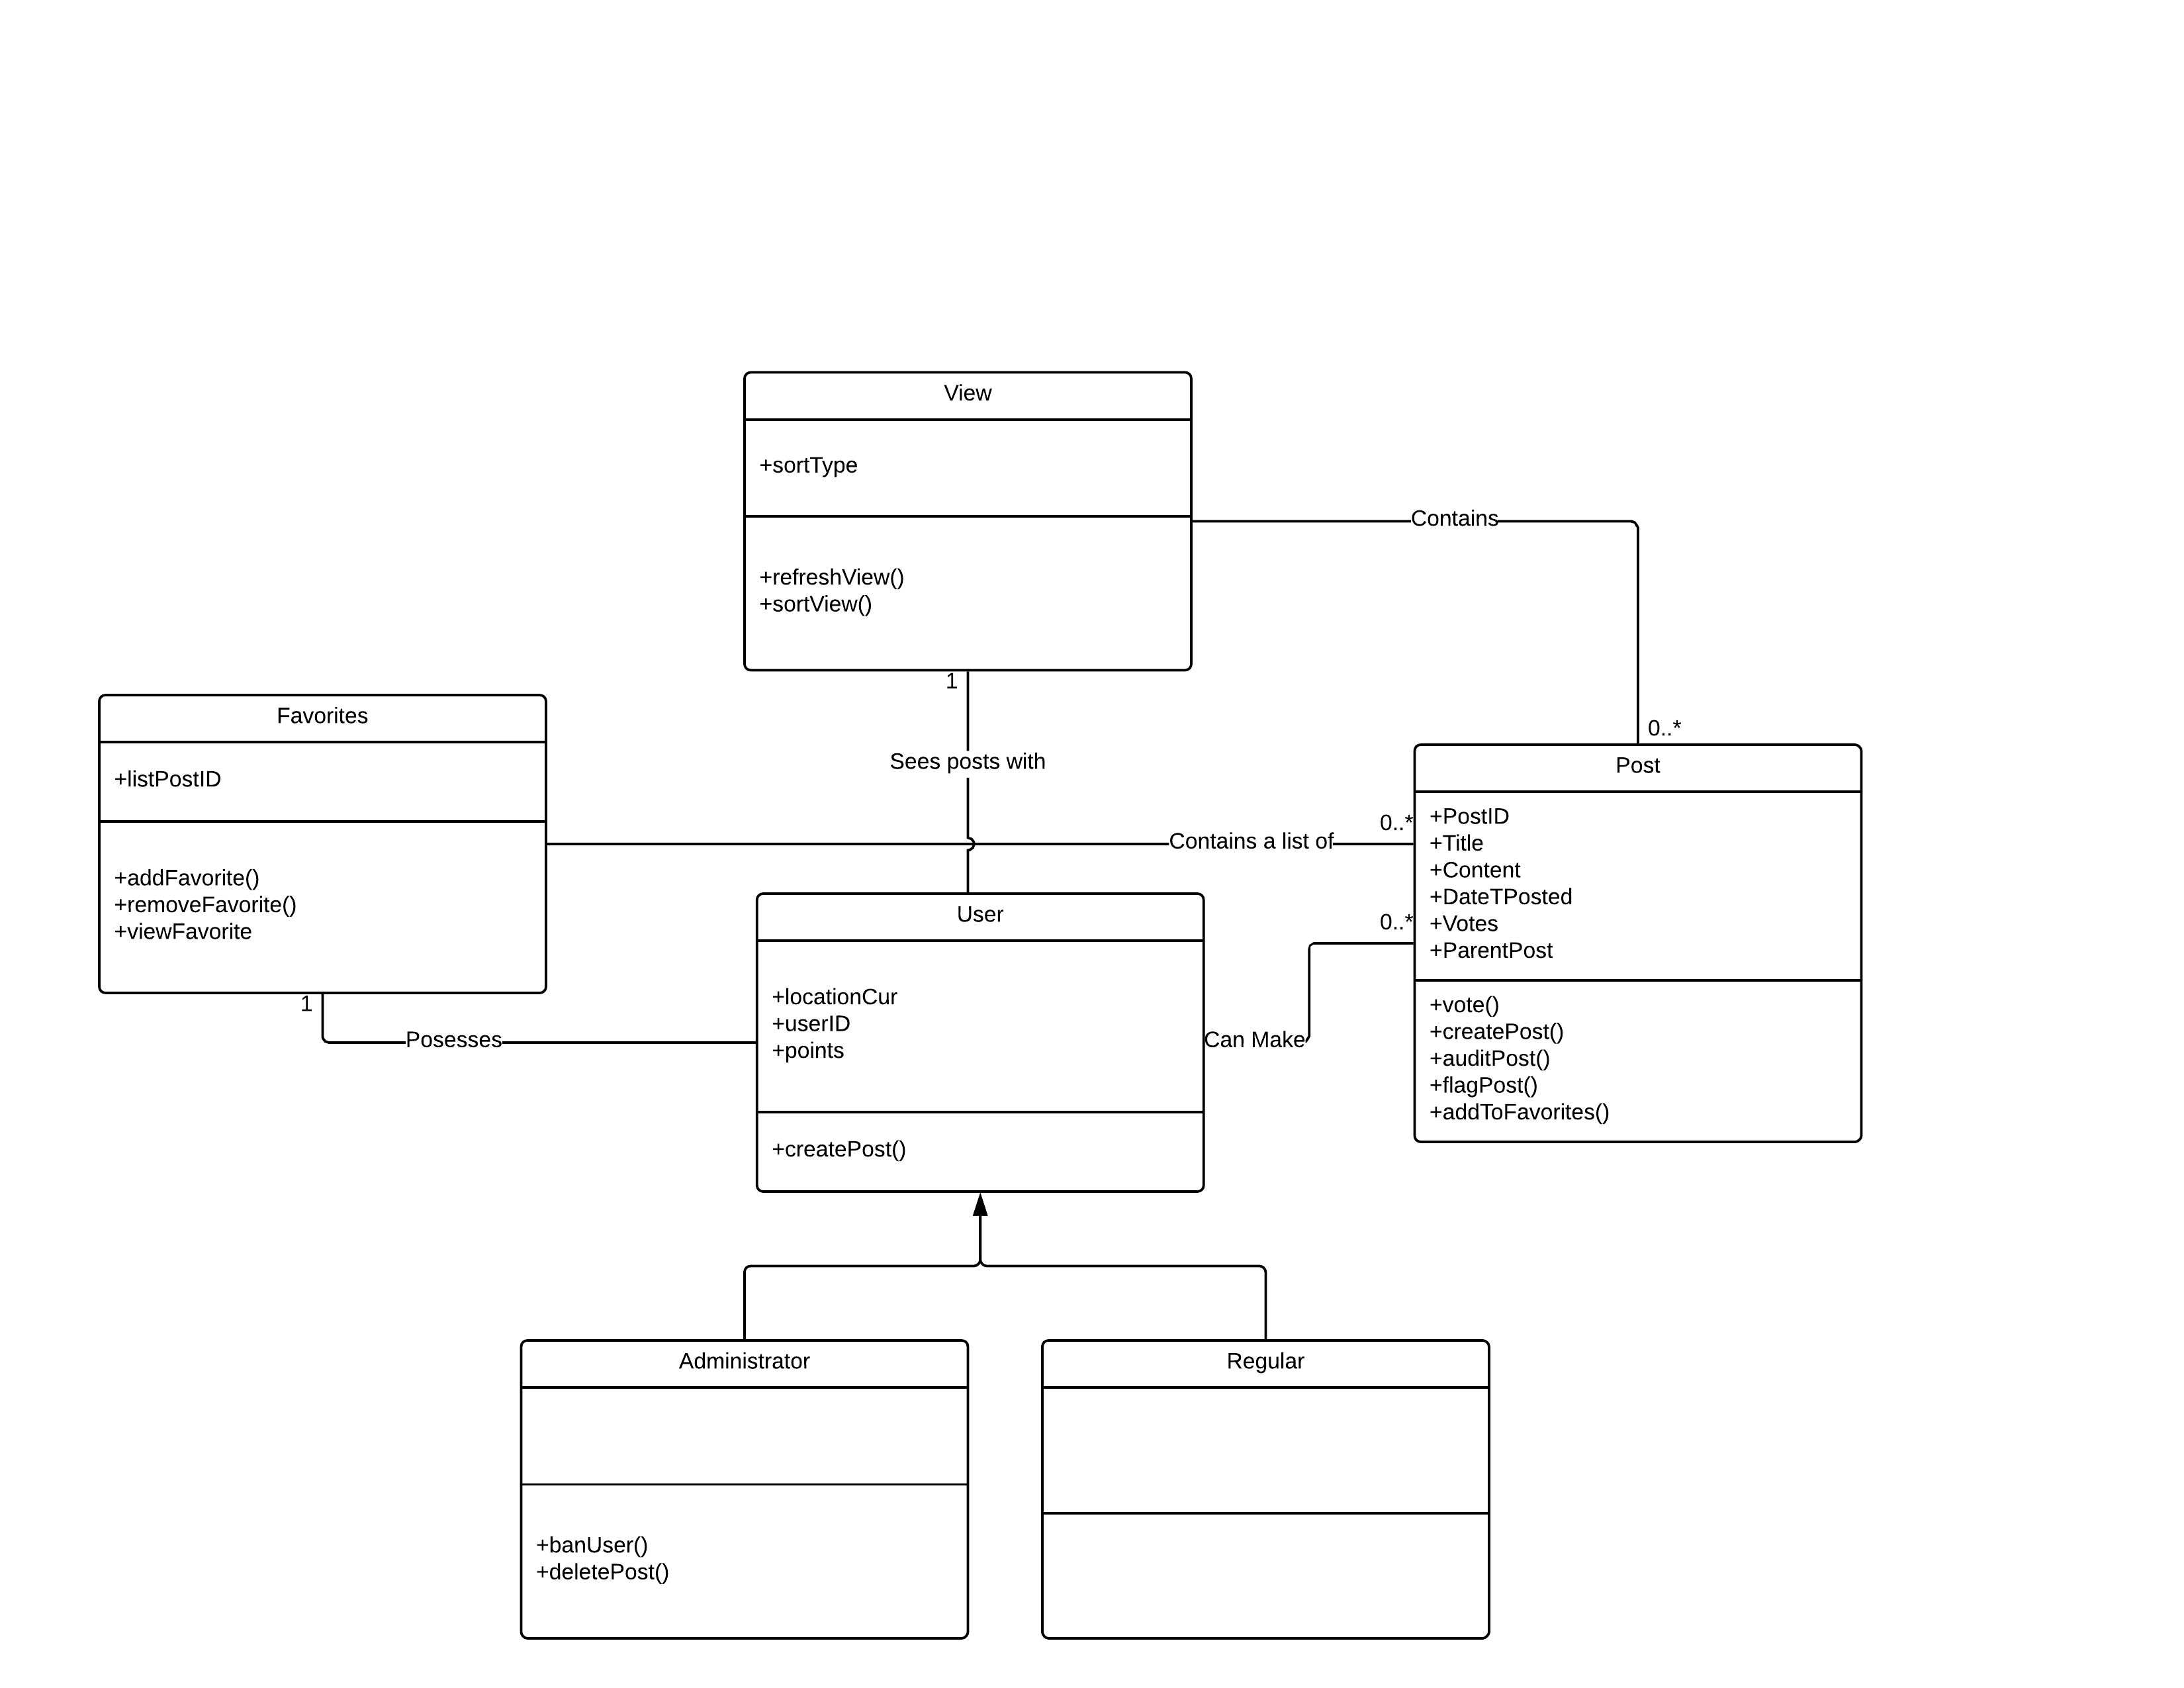
\includegraphics[scale=0.25]{img/uml/ClassDiagram}\linebreak
\textbf{Class Diagram}
  \end{center}

\section{Packages}

Classes are partitioned into two packages- User Package and Posts Package.

\begin{center}
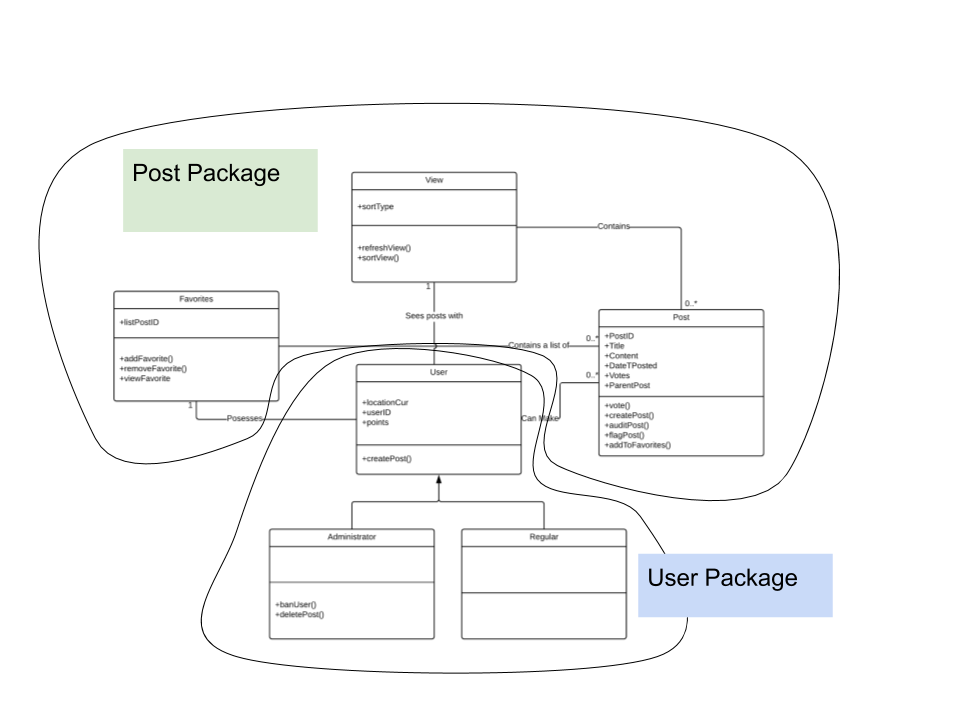
\includegraphics[scale=0.25]{img/uml/packages}\linebreak
\textbf{Packages}
  \end{center}

\subsection{Coupling and Cohesion}

There is low coupling between the packages and mid to high cohesion within each package.
In Posts Package, both Post and View can be changed without affecting Users. The Post class is largely self contained, with its attributes Post-ID, Title, Content, and DateT not relying on any outside classes. Votes and ParentPost are affected by outside class methods, however they can be tested in unit tests by only involving the Post class. Its Vote(), Post(), and Favorite() methods involve no other packages. Aduit() and Flag() involve the Admin User subclass, however changing the Admin class would not affect the Post class as these methods simply send the Post data to Admin. The View class works only with the Post class. Its state attribute sortType is independent of any other classes, and its methods refresh() and sort() only affect objects of the Post class. Favorites class involves elements in both the Users Package and Posts Package, however all of its methods involve interacting only with Post objects. Because the main function of the Favorite class is to store a list of Post objects, it is largely unaffected by the User Package and is not affected by the View Class. Changes to the Post class only affect Favorites if the PostID attribute is changed or if a Post is deleted.
In User Package, Users (both Admin and Regular) attributes can be changed and tested without affecting any of Post Package’s classes. Parent class User has attributes Location, ID, and Points, which can be changed and tested using only the User class. Admin subclass has methods Ban(), which only affects User objects. Regular Users can create and delete posts, however testing of these methods is the same as testing the Post class independently, except for cases of testing that correct PostIDs and Favorites link back to the User.

\section{Design Patterns}
Our system will use a variety of Design Patterns to make the software components we implement reusable and scaleable.

We have design patterns addressing creation, structure, and behavior. We considered addressing concurrency, but there are no concurrency issues with our application that need to be addressed.

\subsection{Builder Design Pattern}

This design pattern will be used to generate posts and comments as record objects with the appropriate fields under a structure, and pushing those information structures to the central database of posts and comments. This ensures that the post and comment creation is done in an efficient way, and enables the creation of an externally facing API that can utilize these objects.

\subsection{Front Controller}

This design pattern will be used to control user interactions in the web application. It will be implemented as a script that is called on every request of the web application. The pattern would handle all tasks that are common to the web app. Rather than running separate scripts for  every user interaction like posting a post or comment or liking a post, the Front Controller will handle them all.

\subsection{Observer (Publish/Subscribe)}

This design pattern will be used to notify the user of certain events occuring. Examples of this would be a new post to the main page, which will be pushed to the user’s main page, or a comment in a thread to a post the user has created, which will notify the user a new comment on their post. New posts and comments are “published” and users that created them are “subscribed” to events related to them.

\subsection{Template}

This design pattern will be used to define repetitive components that can be substituted into the program using a framework such as handlebars. An example of this is a common header file, with font files and html css script loading lines. These will be isolated and called in each separate html page they apply to. This will increase code reuse and make changes to one portion of the design codebase instantly change all pages to which it applies.

\section{Exceptions and Handling}

\section{Meeting report}
\subsection{Progress Made this Week}

This week we worked on getting the different parts of assignment 4 together and assembling the presentation.  We worked on solidifying the design patterns and strategy to make them clearer for both us the programmers and the customer.  We started thinking about direct coding decisions when it came to handling different types of exceptions that may come up.  Additionally we compacted everything into a slide show and practiced presenting in preparation for either tuesday or thursday.

\subsection{Plans for Next Week}

Next we will start nailing down individual user stories for different actions that a user can do.  This will include making a post, voting on a post, fetching a posts or moderating posts.  This will enable us to better plan how to implement these features.  We will also start preparing to program by setting up the toolchain and agreeing on a coding style.

\subsection{Team Member Contributions}

UML Class Diagram - Brendan Byers

Packages - Iliana Javier

Design Patterns - Aiden Grimshaw

Exceptions & Handling - Yufei Zeng

Meeting Report - Brendan Byers

Requirement and Design Presentation - Ryan Sisco, Aiden Grimshaw, Yufei Zeng, Iliana Javier, Brendan Byers 



\end{document}
